\section{Influence Propagation}
\label{sec:influ}

As discussed in Section~\ref{sec:meth}, many files are submitted to VirusTotal more than once, 
and more than 99\% submissions are analyzed by at least 50 anti-virus engines. 
We observe that some engines fail to identify some malwares during early submissions, 
but they catch up when analyzing later submissions. 
Anti-virus vendors frequently use VirusTotal to identify false negatives in their products, 
which are malwares they fail to detect but detected by other vendors. 
We hypothesize that there are influence among different anti-virus vendors.
This section presents our verification of this hypothesis by modeling the cross-vendor influence.
We also provide the prediction model of whether an engine will identify a file as malware in the future
after labeling the file as benign.

\subsection{Influence Model}
\label{sec:model}
Influence propagation on social graph is a well-studied topic in the web mining area. 
Borrowing this idea, we use graphs to represent the relationship between vendors 
and model influence among different vendors based on static models 
originally proposed to analyze Flickr data~\cite{Influence}.
We now explain our graph-based model for anti-virus vendor influence.
% first overview static models in our usage scenario,
%and then we discuss how we evaluate static models on data we collect. 

We first connect all vendors with a complete directed graph $G = (V, E)$, 
where the nodes $V$ are vendors. 
The graph is complete because we assume that influence from any vendor to any other vendor is possible.
We define an action ($a$) at time $t$ as $(u, a, t)$ or $(u, \bar{a}, t)$,
as the former represents an anti-virus engine identifies the submission as malware 
and the latter represents it identifies the submission as benign.
Since the goal of our study is to detect if the change from labeling a file as benign to labeling it as malware by a vendor is influenced by other vendors, 
we do not consider the case of changing from labeling benign to malware and assume that after a vendor labels a file as malware, it will not change its decision.
A similar model can be applied to study the latter type.

We associate each edge $(u, v) \in E$ in the graph $G$ 
with an influence probability $p_{u,v}$,
which represents the probability that after $u$ takes an action $v$ will follow $u$ to take the same action.
We only consider cases of changing from labeling benign to malwares, 
which means that when calculating $p_{u,v}$, we only consider cases where $u$ has labeled a submission as malware, 
$v$ will label a submission as malware in the future, 
and $v$ labeled the submitted file as benign earlier. 
%\yiying{does this action include both turning from labeling benign to malware and from malware to benign? 
%does it include the first label (no prior labeling by the same node)? you need to explain what an "action" is.}
%Since the graph is a complete graph, 
%all other nodes are all $v$'s neighbors. 
For an action $a$, we use $S_v(a)$ to represent the set of $v$'s neighbors taking action $a$ before $v$ in time. 
The probability that $v$ will follow its neighbors to take the same action can then be calculated as:

\begin{equation} \label{eq:setp}
%$$p_v(S_v(a)) = 1 - \prod\limits_{u \in S_v(a)}(1 - p_{u,v})$$
p_v(S_v(a)) = 1 - \prod\limits_{u \in S_v(a)}(1 - p_{u,v})
\end{equation}

Thus, if we know the probability of a node influencing another node ($p_{u,v}$) for all node pairs,
we can know the probability of a node (an anti-virus vendor) being influenced by other nodes (other anti-virus vendors).
The goal of our learning model is thus to estimate $p_{u,v}$.

Specifically, during training stage, we learn $p_{u,v}$ for each edge. 
We designed four static models for the training stage, which differ in how to estimate $p_{u,v}$ by using the data in training set. 

During prediction stage, we test a node $v$ that has not taken the action $a$ yet
and predict if it will take this action following other nodes. 
Specifically, we use a tunable threshold $\theta$
and predict $v$ will follow its neighbors to take the action $a$ in the future
if $p_v(S_v(a))>\theta$.

Before delving into the details of how our four static models estimate $p_{u,v}$ during the training stage, 
we first gives a set of definitions that we make to assist the development of these models.
We use $A_u$ to represent the set of submissions identified by $u$ as malwares in its history
and $\bar{A}_u$ represents the set of submissions ever labeled as benign by $u$.
%the number of actions taken by $u$, 
%or the number of malwares identified by $u$. 
%\yiying{I think all these $A$ should be a collection/set, not the total number, since you use $\in$ later}
%\yiying{Verify that the above sentence is correct.}
Further, we define the set of actions taken by both $u$ and $v$ as $A_{u\&v}$ 
and the set of actions taken by either $u$ or $v$ as $A_{u|v}$.
Thus, $|A_{u|v}| =   |A_u| + |A_v| - |A_{u\&v}|$.

Finally, we define {\em action propagation} as follow and use $A_{u2v}$ to represent the set of all the actions that are propagated from $u$ to $v$. 

\begin{definition}{Action Propagation:}
We say that an action $a$ propagated from $u$ to $v$ iff: (i) $\exists$ $(v, \bar{a}, t_i)$ $\in$ $\bar{A}_v$ 
and $(v, a, t_k)$ $\in$ $A_v$, with $t_i < t_k$; (ii) $\exists$ $(u, a, t_j)$ $\in$ $A_u$, with $t_j < t_k$ and $u \neq v$. 
\end{definition}

With these definitions, we now present our four static models.

{\bf Bernoulli distribution} estimates $p_{u,v}$ as the ratio of the number of actions 
propagated from $u$ to $v$ over the total number of actions taken by $u$.

$$p_{u,v} = \frac{|A_{u2v}|}{|A_u|}$$ 

{\bf Jaccard index} estimates 
$p_{u,v}$ as the number of actions propagated from $u$ to $v$ divided by 
the number of actions taken either by $u$ or by $v$.

$$p_{u,v} = \frac{|A_{u2v}|}{|A_{u|v}|}$$ 

On top of the Bernoulli distribution and the Jaccord index,
we add an additional consideration called {\em partial credit}.
When $v$ takes an action $a$, it may be influenced by the combination of all its neighbors $S_v(a)$ 
taking the action $a$ before $v$. %Partial credit takes this intuition. 
To account for this effect, we use partial credit 
and calculate the partial credit for $u$ who takes an action $a$ before $v$ as 

$$credit_{u,v}(a) = \frac{1}{|S_v(a)|}$$

{\bf Bernoulli distribution with partial credit} 
estimates $p_{u,v}$ as the sum of all partial credits taking by $u$ for actions propagated from $u$ to $v$, 
dividing by the number of actions taken by $u$. 

$$p_{u,v} = \frac{\sum\limits_{a \in A_{u2v}}{credit_{u,v}(a)}}{|A_u|}$$

{\bf Jaccard index with partial credit} 
estimates $p_{u,v}$ as the sum of all partial credits taking by $u$ for actions propagated from $u$ to $v$, 
dividing by the number of actions taken either by $u$ or by $v$. 

$$p_{u,v} = \frac{\sum\limits_{a \in A_{u2v}}{credit_{u,v}(a)}}{|A_{u|v}|}$$




\subsection{Model Evaluation}
\label{sec:predict}

\noindent{\underline{\textit{Training stage methodology.}}}
We split all the \pe\ submissions we collected into a training set and a testing set based on the SHA256 values of the submitted files. 
We place all submissions with SHA256 values starting with a numeric character, 
i.e., from ‘0’ to ‘9’, into training set
and all the rest into the testing set.

We implement the training process by several stages of map, filter, and reduce in Spark. 
Specifically, we first reduce submission records according to submitted files. 
We then sort submission records chronologically.
For each remaining file, we compute four maps based on its submissions.
There is one one-dimension map, 
containing the number of actions taken by each vendor, 
or the number of malwares identified by each vendor. 
There are three two-dimension maps, 
containing an entry for each pair of vendors $(u,v)$, 
representing actions taken by both $u$ and $v$, actions propagated from $u$ to $v$, 
and partial credits taken by $u$ for actions propagated from $u$ to $v$. 
Finally, we reduce these 4 maps from different files, 
and calculate $p_{u,v}$ for the four static models. 

After training the four static models, 
we filter out engines taking fewer than 10000 actions,
since engines taking too few actions cannot produce meaningful results.
There are 59 engines left
and the average number of actions taken by these engines is around 190K. %190140, which is much larger than 10000.
For confidentiality reasons, we omit vendors’ name in the following discussion
and use numbers from 0 to 58 to represent these vendors.

\noindent{\underline{\textit{Training results.}}}
For each static model, 
we put all learned $p_{u,v}$ in a influence table, 
by using $u$ as row number and $v$ as column number.
For any $p_{u,v}$, Bernoulli distribution has the largest value, 
Jaccard index has the second largest value, 
Bernoulli with partial credit has the third largest value,
and Jaccard index with partial credit has the least value. 

\begin{figure*}
\centering
\subfloat[]{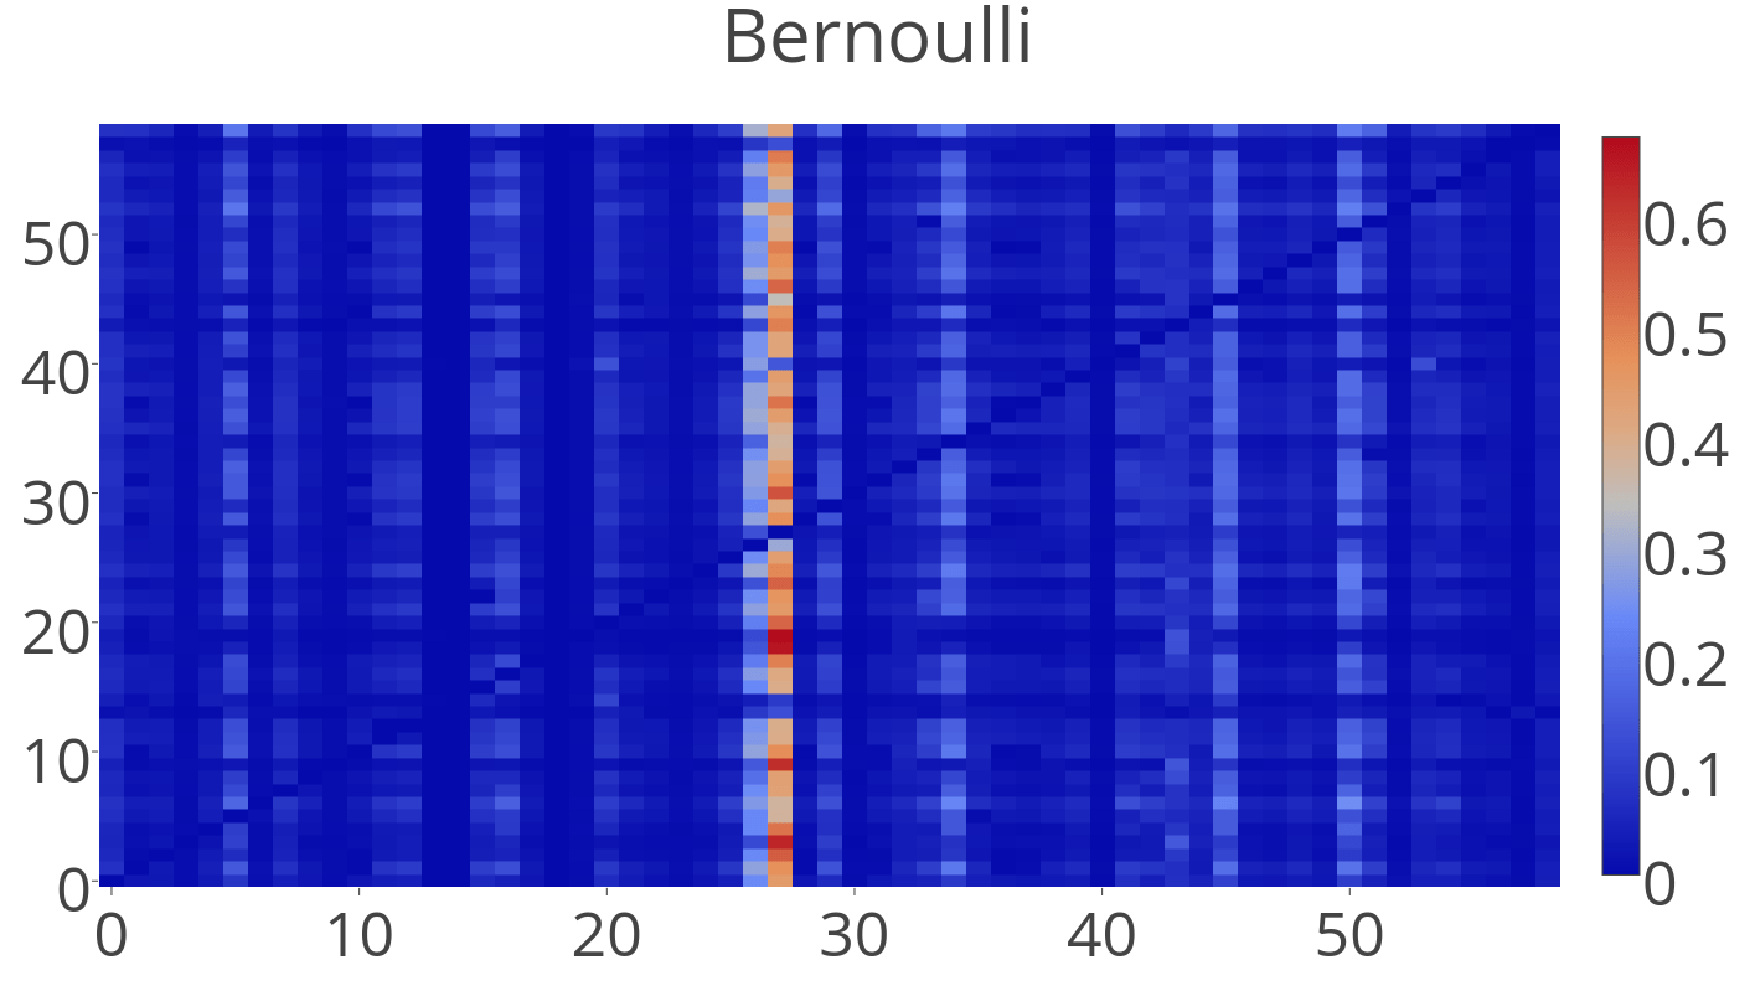
\includegraphics[width=0.24\linewidth]{figure/bernoulli-train}\label{fig:moredata1}} 
\subfloat[]{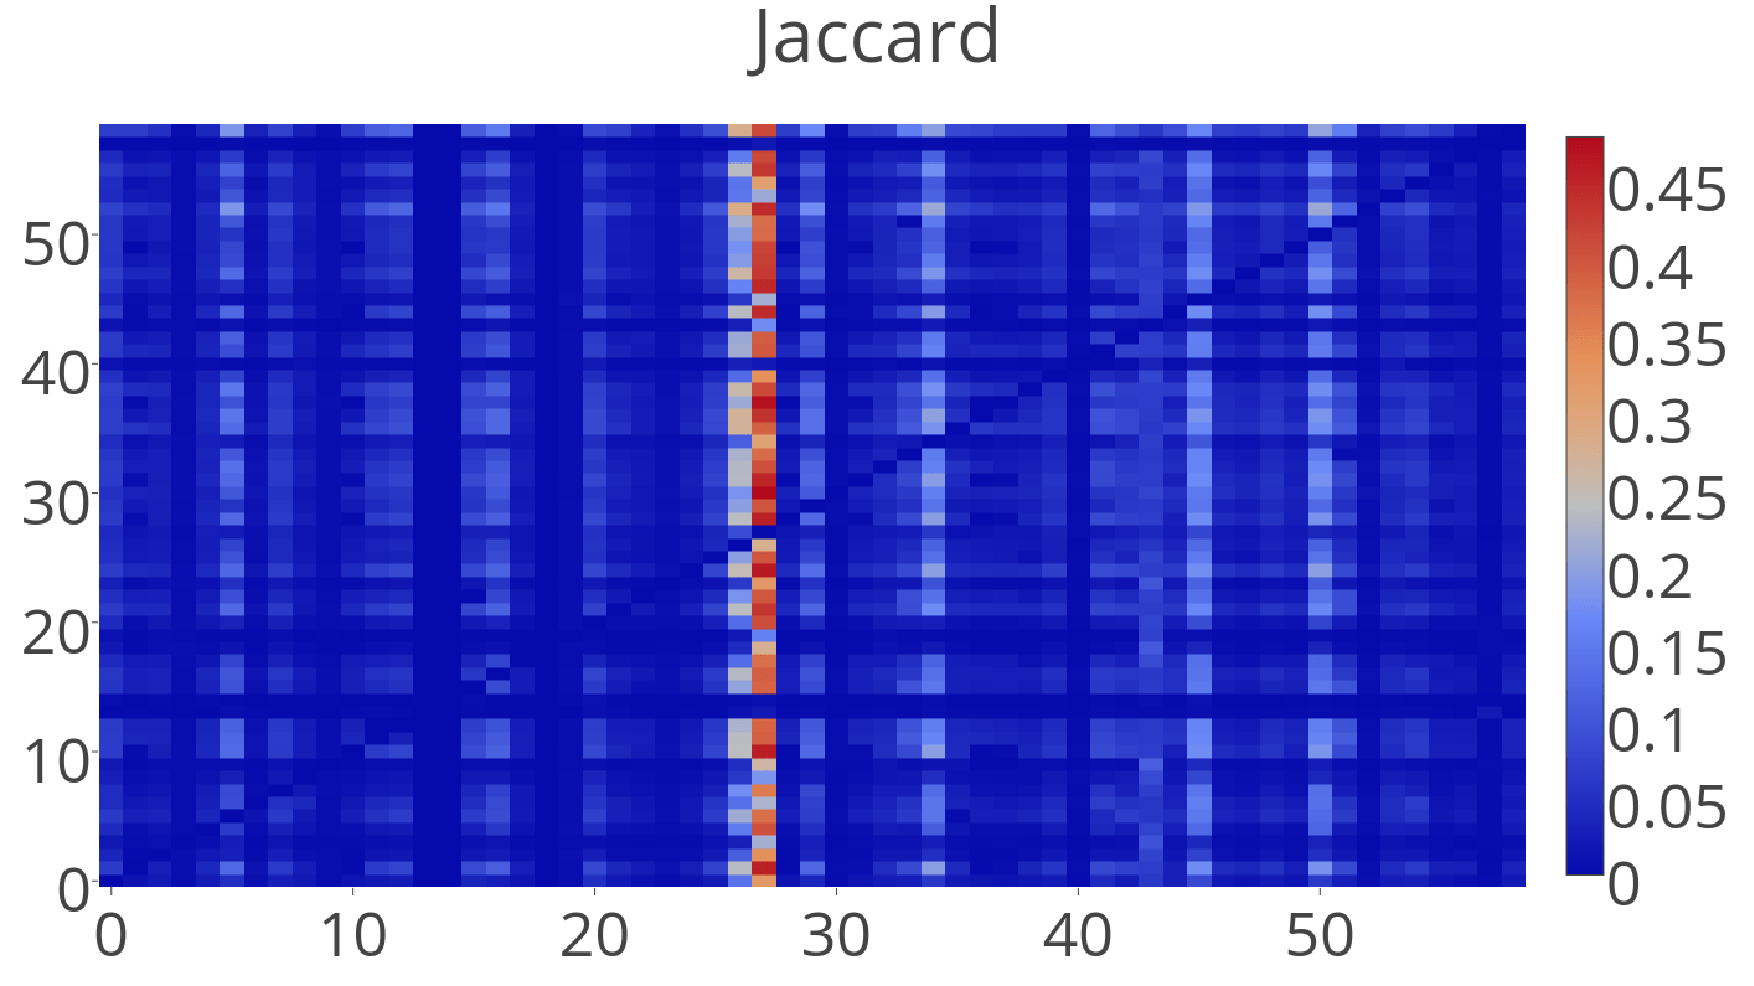
\includegraphics[width=0.24\linewidth]{figure/jaccard-train}\label{fig:moredata2}}
\subfloat[]{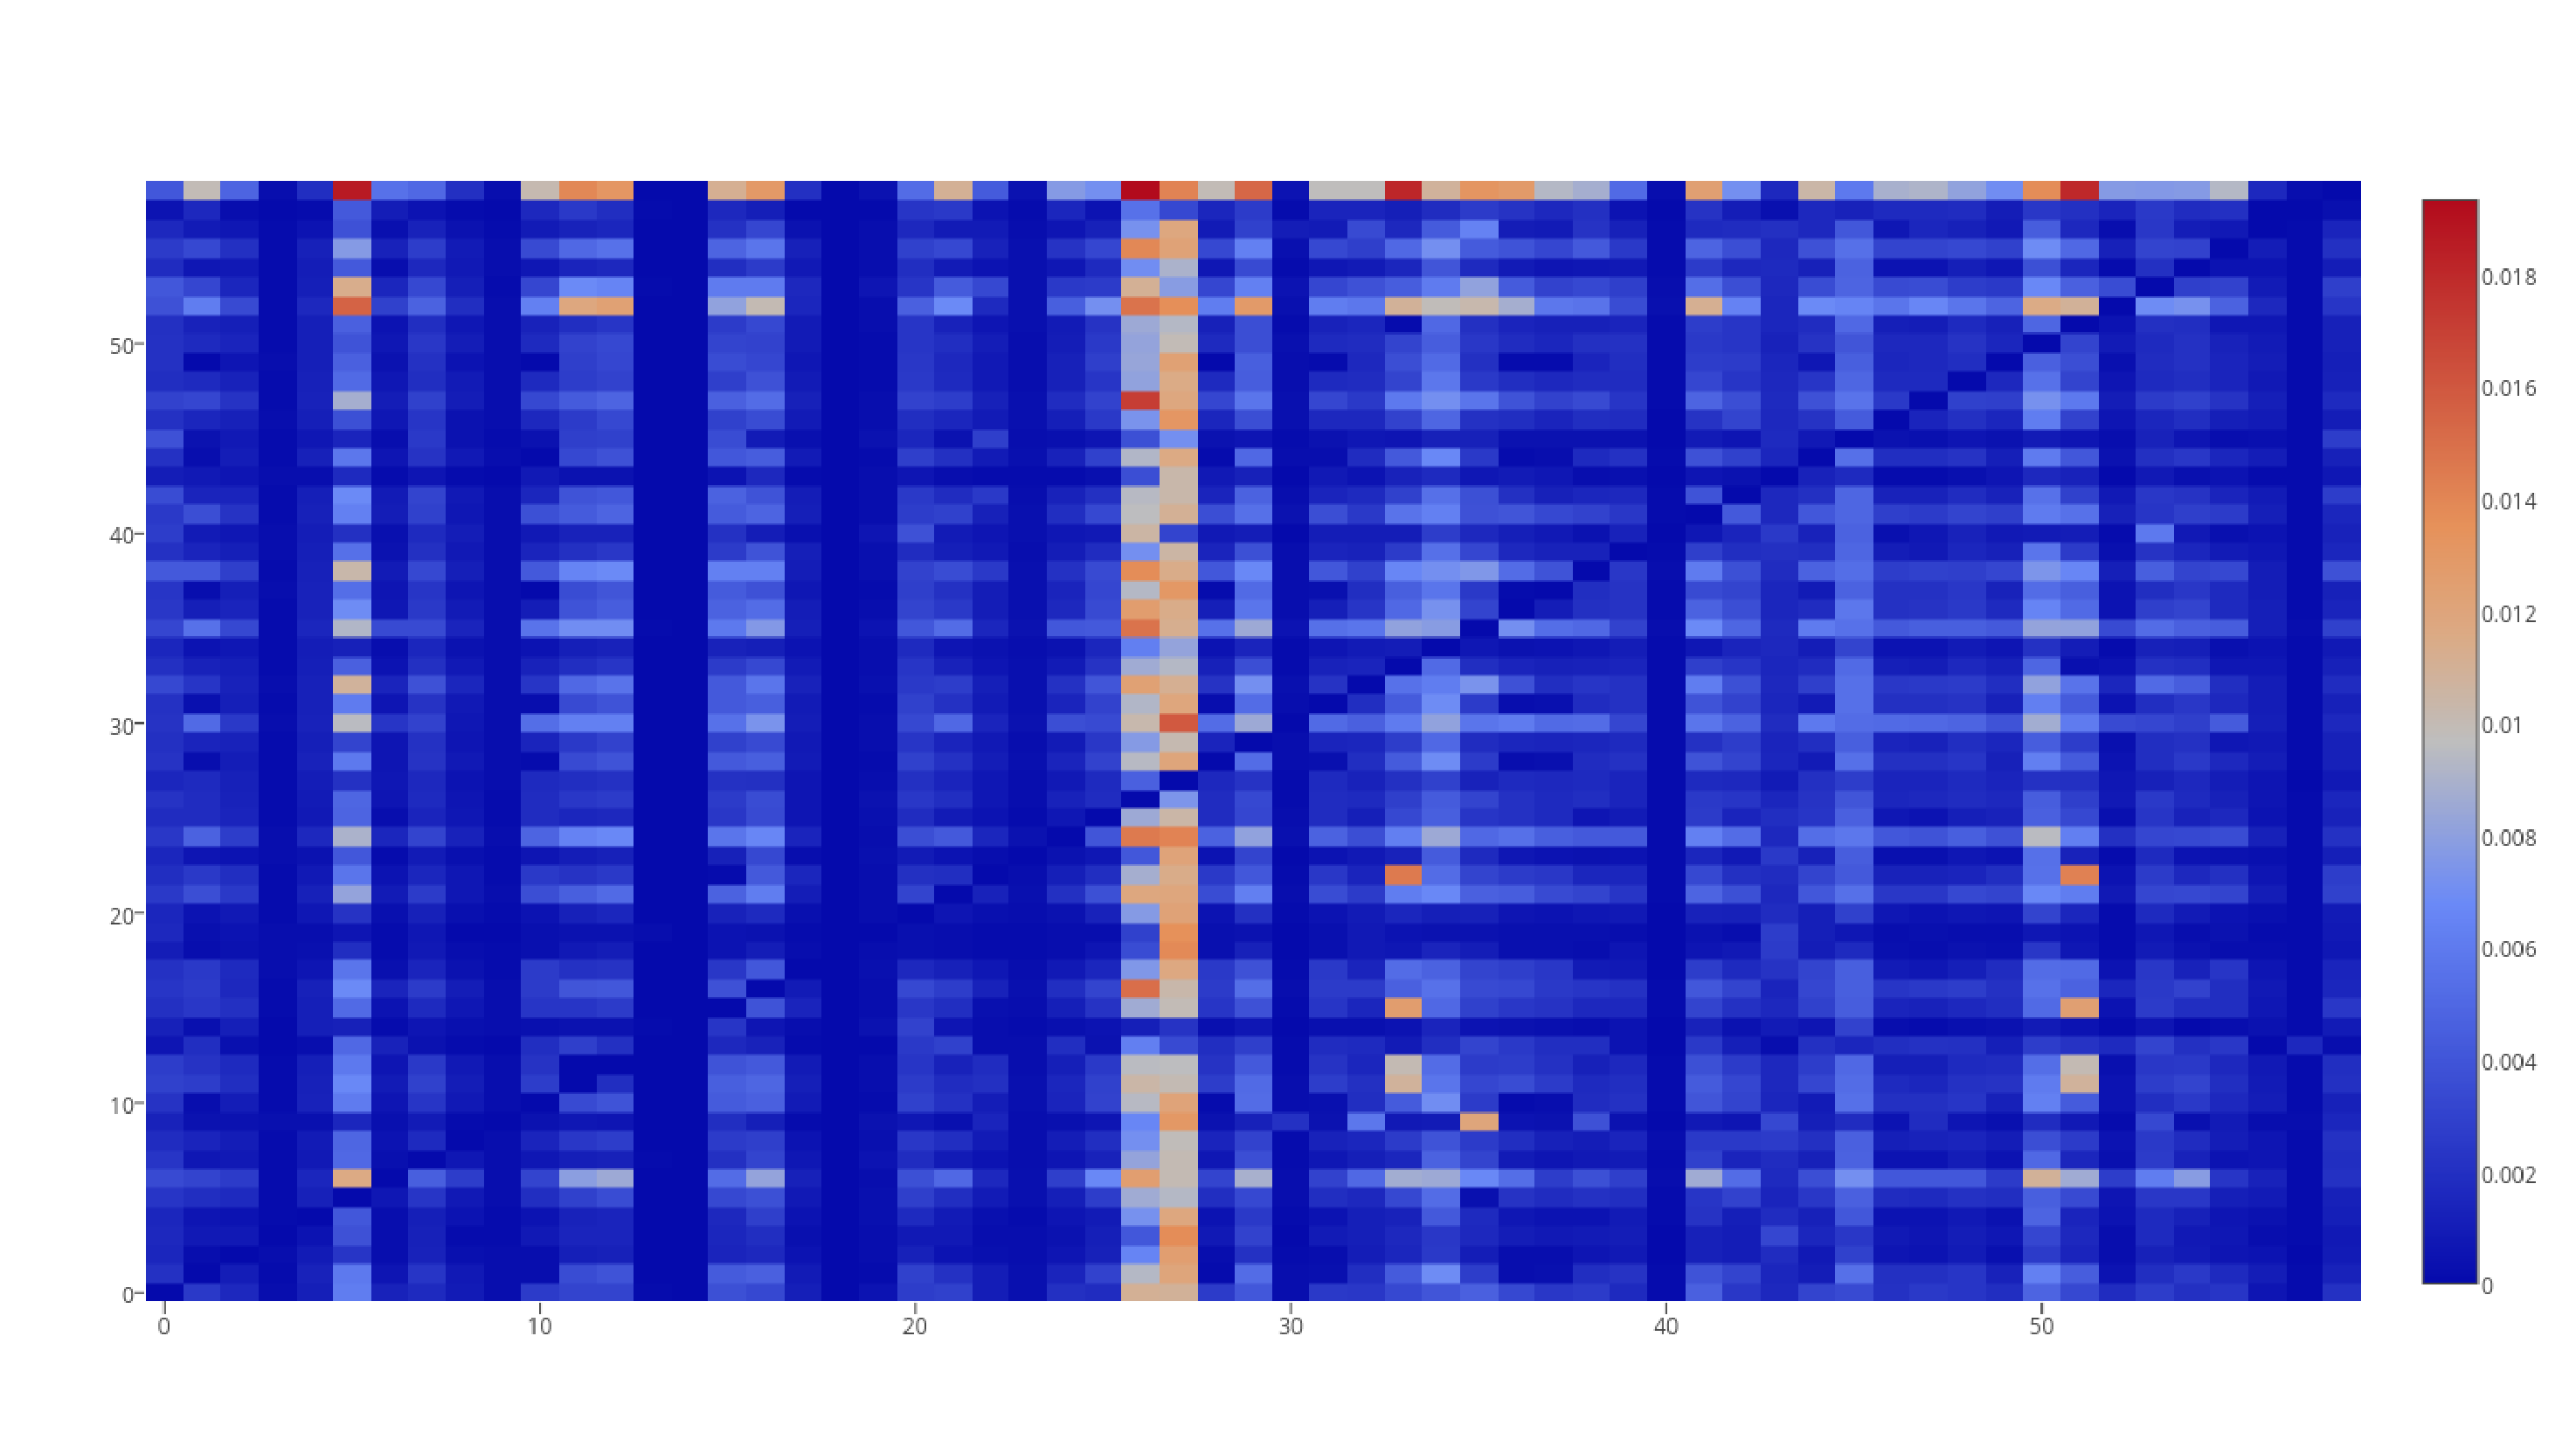
\includegraphics[width=0.24\linewidth]{figure/PC-train}\label{fig:moredata3}} 
\subfloat[]{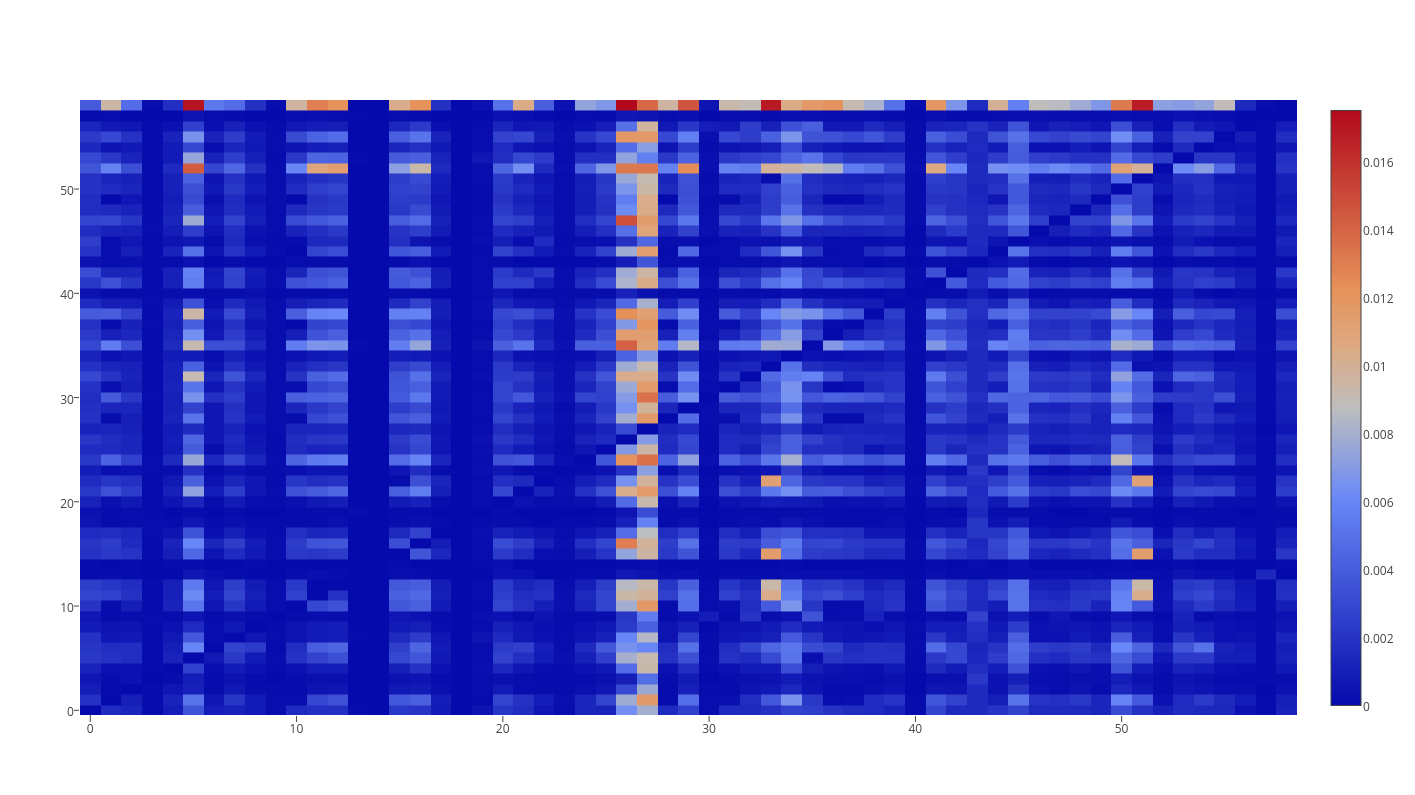
\includegraphics[width=0.24\linewidth]{figure/jaccardPC-train}\label{fig:moredata4}} \\ 
\caption{Potential for 0.5 V bias.} 
\label{fig:EcUND} 
\end{figure*} 


\begin{figure}[t!]
\begin{center}
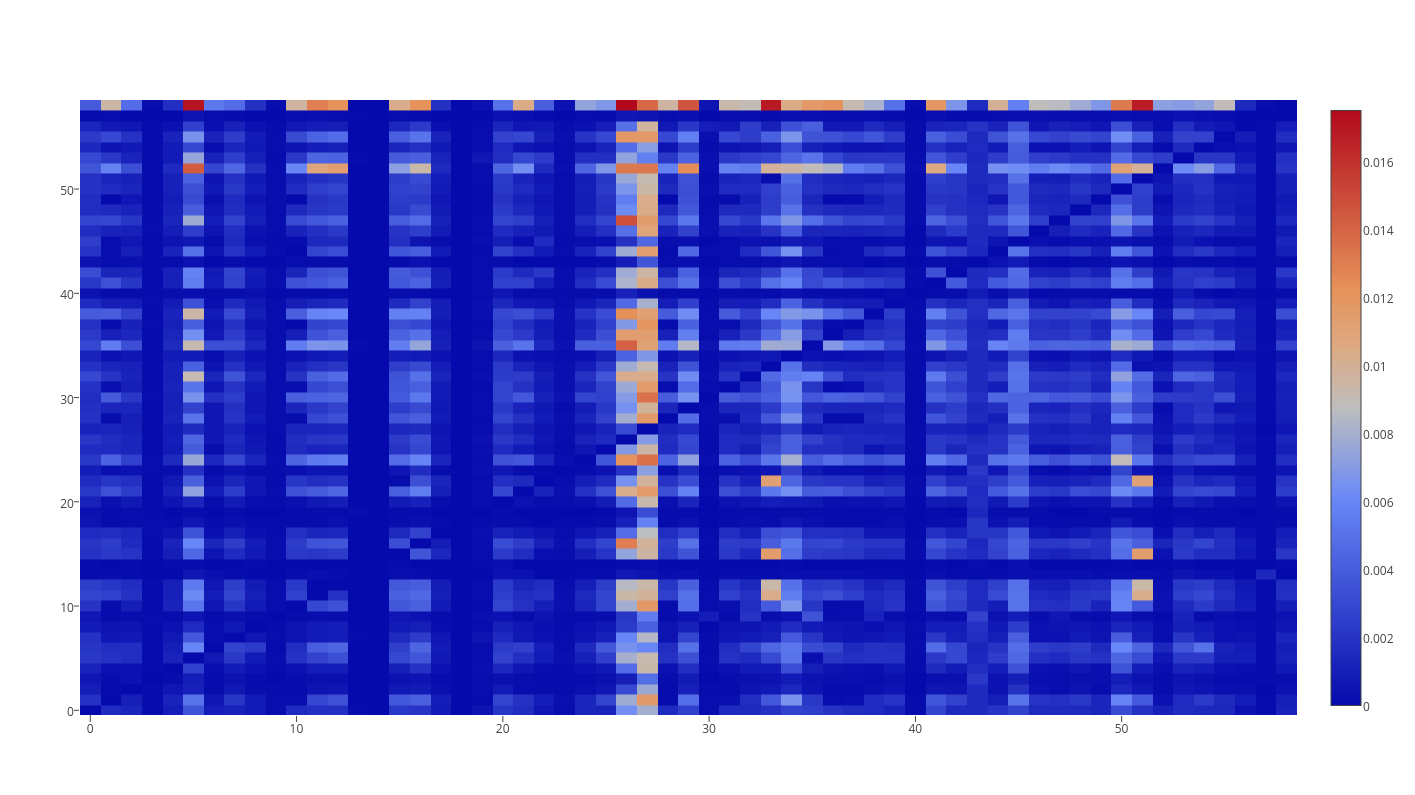
\includegraphics[width=2.5in]{figure/jaccardPC-train}
\mycaption{fig:idreputation}{Test.}
{\footnotesize{(How detection rate changes with the value of source id's reputation. Each reputation is rounded up to nearest 0.05.
Reputation -1 means the source id did not make any submission before. 95\% confidence interval is also drawn 
for each point.)}}
\end{center}
%\vspace{-0.25in}
\end{figure}

We draw heat maps for all learned influence tables in Figure~\ref{fig:heat}. 
Given a $cell(u, v)$ with $u$ as row number and $v$ as column number, 
red color means more influence from $u$ to $v$. 
The four heat maps share a similar pattern.
There are columns with almost all cells in red color, 
which means there are vendors influence by all other vendors. 
There are no rows with all cells in red color, 
and this means that there are no vendors which can influence all other vendors. 

For each row in all influence tables, we sum all its number together. 
The results can serve as a quantitative measurement for engines' influence in malware detection community. 
Influence rankings from all the four static models also share a similar pattern. 

{\bf Observation 7:} 
{\em Certain anti-virus vendors are influenced by all other vendors in their malware detection decision.}

\noindent{\underline{\textit{Testing stage methodology.}}}
We also used Spark to implement the testing process and express the process using several stages of map, filter, and reduce.
Similar to our training stage process, 
we first reduce all submissions based on submitted files,
next filter out files without action propagation, 
and then sort submissions chronologically. 

To test a submission, we first use Equation~\ref{eq:setp} to
calculate $p_v(S_v(a))$ for all engines
that labeled the submitted file as benign when analyzing early submissions 
but have not labeled the file as malware. 
$S$ is the set of engines which labeled the file as malwares before.
We compare $p_v(S_v(a))$ with a given threshold $\theta$ to decide whether we predict 
$v$ will label the file as malware.
We then check what $v$ actually labels in the submission to count true positive (TP) and false negative (FN). 
After processing all submissions for a file, 
we calculate $p_v(S_v(a))$ for all engines  
that label the file as benign but have not labeled the file as malware.
We compare $p_v(S_v(a))$ with $\theta$ to count false positive (FP) and true negative (TN).
In the final stage, we reduce TP, TN, FP, and FN numbers from different files.

\begin{figure}[t!]
\begin{center}
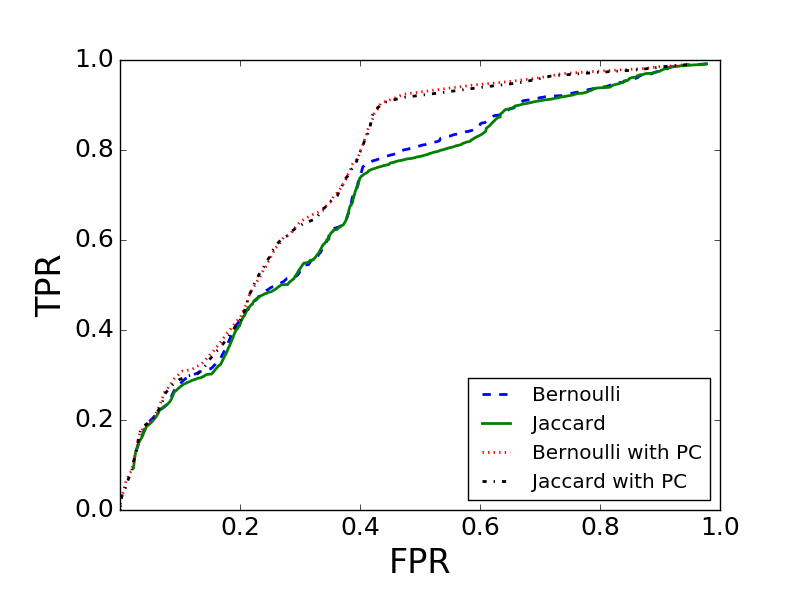
\includegraphics[width=2in]{figure/predict}
\vspace{-0.1in}
\caption{ROC comparisons of Static Models. 
(How true positive rate (TPR) changes with false positive rate (FPR). 
We change probability threshold from 0.1\% to 99.9\% with step 0.1\%. 
We compute TPR and FPR for each probability threshold to draw the curve.)
}
\label{fig:predict}
\end{center}
\vspace{-0.1in}
\end{figure}

\noindent{\underline{\textit{Testing results.}}}
We change the probability threshold $\theta$ from 0.1\% to 99.9\% 
and 
%by using 0.1\% as step. 
We measure the accuracy of the four static models using ROC (Receiver Operating Characteristic) curves,
with true positive rate ($TPR = TP/(TP+FN)$) as X-axis
and false positive rate ($FPR = FP/(FP + FN)$) as Y-axis. 
Figure~\ref{fig:predict} plots the ROC curves for the four static models.
The larger the area under the ROC curve, the better the performance.
We find that, all models beat random guesses
(the diagonal line between (0,0) to (1,1)) significantly. 
Using partial credits improves the accuracy of both Bernoulli and Jaccard index.

{\bf Observation 8:} 
{\em The influence model borrowed from
social media analysis contains information
that helps the prediction of the temporal
behavior of malware detection. }

\subsection{Discussion}

\if 0
There are also time models proposed by~\citet{Influence}.
When analyzing Flickr data, time models leverage accurate action time to provide better prediction performance. 
However, we do not use time models, 
because time information we access is when a submission is conducted, 
or when an engine analyzes a submission, 
is not when an engine changes its detection label for a file.
The time information we have can only provide a relative order about when each vendor identifies a file as a malware.  

\underline{Limitation.}
Our data collection ends on 09/06/2016. 
We could count extra FPs, where we predict engines will label files as malwares, engines have not, but will do in the future, 
and TNs, where we predict engine will not label, engines have not, but will in the future. 
Monitoring \vt for a longer time will make the evaluation of our prediction models more precise. 

\underline{How to use?}
\fi

Our findings in this section rings an alert toward using detection rate as the pure measurement of the likelihood of a file being malware
and shed light on how vendors can influence each other.
Our study results can serve as a quantitative measurement for vendors' influence in malware detection community. 
Previously, when combining results from different vendors, 
security experts simply treat each vendor equally and use the percentage of 
vendors labeling a file as malware as likelihood of the file to be a malware. 
Our model can provide a weight, when combining results from different vendors.  
For anti-virus vendors, the prediction part of our models can help alarm possible false negatives in their products.
